\documentclass[11pt]{article}

\usepackage[a4paper,margin=1in]{geometry}
\usepackage[utf8]{inputenc}
\usepackage{tikz}
\usetikzlibrary{positioning,arrows.meta,fit,backgrounds,calc}
\usepackage{booktabs}
\usepackage{listings}
\usepackage{xcolor}
\usepackage{hyperref}
\usepackage{caption}
\usepackage{subcaption}
\usepackage{graphicx}
\usepackage{amsmath}
\usepackage{amssymb}
\usepackage{enumitem}
\usepackage{parskip}

\hypersetup{colorlinks=true, linkcolor=blue, urlcolor=blue, citecolor=blue}

\lstset{
  basicstyle=\ttfamily\small,
  breaklines=true,
  columns=fullflexible,
  frame=single,
  backgroundcolor=\color{gray!8},
  showstringspaces=false,
}

% ---------------------------------------------------------------------
% Placeholder helpers -- search for \screenshot{ and \fillin{ to find
% every spot that still needs something inserted by hand (a screenshot,
% a name, a group-specific detail).
% ---------------------------------------------------------------------
\newcommand{\screenshot}[2][4.6cm]{%
  \begin{center}
  \begin{tikzpicture}
    \node[draw, dash pattern=on 6pt off 4pt, very thick, color=gray!70,
          rounded corners=4pt, minimum width=0.85\textwidth, minimum height=#1,
          align=center, text width=0.78\textwidth, inner sep=8pt] {%
      \color{gray!80}\Large $\boxtimes$\\[0.4em]
      {\color{gray!90}\bfseries\large INSERT SCREENSHOT HERE}\\[0.35em]
      {\color{gray!70}\normalsize\itshape #2}
    };
  \end{tikzpicture}
  \end{center}
}

\newcommand{\fillin}[1]{\textcolor{red!70!black}{\texttt{[FILL IN: #1]}}}

\title{
\includegraphics[width=2.6cm]{Images/buet_logo.png}\\[0.6em]
{\Large CSE406: Cyber Security Sessional}\\[0.3em]
{\LARGE TCP Reset Attack on Video Streaming}\\[0.3em]
{\large Final Report --- Project Tool \#15}}
\author{2105094: Omar Abdur Razzaque \\ 2105104: Rubaiyat -E-Zaman}
\date{September 19, 2026}

\begin{document}
\maketitle

\begin{abstract}
We implement, from scratch, a TCP reset (RST) attack against a video
streaming session: an on-path attacker forges a \texttt{RST} segment
that appears to originate from the legitimate server, using a sequence
number read directly off the victim's own outgoing traffic rather than
guessed, terminating the client's connection and interrupting playback.
We describe the attack's design and implementation, the expected and
actually observed outcomes (including one case where they diverge, and
why), a switch-side countermeasure (IP Source Guard) that defeats the
attack, and quantitative, repeated-trial measurements of both the
attack's success rate and the defense's effectiveness across a range of
network conditions.
\end{abstract}

\tableofcontents

% =======================================================================
\section{Introduction}
% =======================================================================

This report covers the implementation and evaluation of course project
Tool \#15: a TCP reset attack on video streaming. An on-path attacker,
sharing a switched LAN with a video-streaming client, forges a TCP
\texttt{RST} segment that appears to come from the legitimate streaming
server. The forged RST kills the client's connection immediately,
interrupting playback, without guessing any sequence number -- the
value used is read directly from the client's own outgoing traffic.

The rest of this report is organized as follows. Section~\ref{sec:threat}
states the threat model and the assumptions the attack depends on.
Section~\ref{sec:impl} describes the emulated topology and the
implementation of the streaming service and the attacker.
Section~\ref{sec:process} describes the attack process step by step and
the expected outcome. Section~\ref{sec:observed} reports what was
actually observed, both qualitatively (logs, screenshots) and
quantitatively (repeated-trial success rates across network
conditions), and discusses the one case where the observed outcome
diverged from what was expected. Section~\ref{sec:defense} describes and
evaluates a switch-side countermeasure. Section~\ref{sec:discussion}
discusses limitations and scope, and Section~\ref{sec:conclusion}
concludes.

% =======================================================================
\section{Threat Model and Assumptions}
\label{sec:threat}
% =======================================================================

The attacker is \emph{on-path}: it shares the same switched LAN segment
as the video-streaming client, while the real streaming server is
remote, reachable only through a router. The attacker does not suppress,
delay, or otherwise interfere with legitimate traffic -- it only
observes the client's traffic and injects forged packets alongside it.
The target is the TCP layer, independent of the HTTP version in use.

\paragraph{Explicit assumption: on-path visibility.} A switched LAN does
not, by default, deliver one host's unicast traffic to another host on
the same switch. Real-world attackers typically obtain this visibility
via ARP spoofing, which poisons the ARP caches of the client and its
gateway so that frames addressed to each other are instead delivered to
the attacker. \textbf{This project explicitly assumes that this
precondition has already been satisfied} by the time the attack begins.
ARP spoofing itself is a separately assigned project tool (Tool \#1),
and reimplementing it here would duplicate that tool's scope rather than
demonstrate the RST-specific mechanics this tool is graded on. In the
emulated topology (Section~\ref{sec:impl}), we reproduce ARP spoofing's
\emph{data-plane consequence} -- the attacker being able to see the
client's traffic -- directly, via a switch port mirror, rather than by
performing the spoofing itself.

\paragraph{Other assumptions.} The server is assumed to be running an
ordinary HTTP/1.1 streaming service (no custom protocol hardening beyond
what a standard Linux TCP stack already provides, e.g.\ RFC 5961
protections, which are discussed explicitly in
Section~\ref{sec:observed}). Only \emph{Attack A} -- a forged RST
delivered to the \emph{client}, spoofed as the server -- is implemented
and evaluated; the converse (spoofing the client toward the server) is
architecturally straightforward given the same sequence-number-inference
trick, but is not required and not evaluated here.

% =======================================================================
\section{Topology and Implementation}
\label{sec:impl}
% =======================================================================

\subsection{Network Topology}

The entire topology is emulated in code using Mininet and Open vSwitch
-- no physical or virtual routers/switches, and no separate virtual
machines. Figure~\ref{fig:topology} shows the layout.

\begin{figure}[h]
\centering
\resizebox{0.9\textwidth}{!}{%
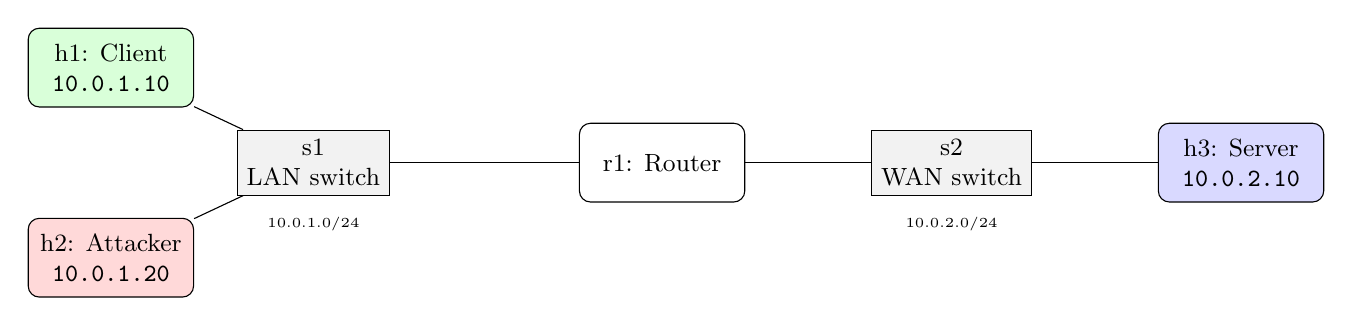
\begin{tikzpicture}[
    node distance=1.4cm and 1.6cm,
    host/.style={draw, rounded corners, minimum width=2.1cm, minimum height=1cm, align=center, font=\small},
    sw/.style={draw, rectangle, minimum width=1.6cm, minimum height=0.8cm, align=center, font=\small, fill=gray!10},
  ]
  \node[host, fill=green!15] (h1) {h1: Client\\ \texttt{10.0.1.10}};
  \node[host, fill=red!15, below=of h1] (h2) {h2: Attacker\\ \texttt{10.0.1.20}};
  \node[sw, right=of $(h1)!0.5!(h2)$] (s1) {s1\\LAN switch};
  \node[host, right=2.4cm of s1] (r1) {r1: Router};
  \node[sw, right=of r1] (s2) {s2\\WAN switch};
  \node[host, fill=blue!15, right=of s2] (h3) {h3: Server\\ \texttt{10.0.2.10}};

  \draw (h1) -- (s1);
  \draw (h2) -- (s1);
  \draw (s1) -- (r1);
  \draw (r1) -- (s2);
  \draw (s2) -- (h3);

  \node[below=0.15cm of s1, font=\tiny] {10.0.1.0/24};
  \node[below=0.15cm of s2, font=\tiny] {10.0.2.0/24};
\end{tikzpicture}%
}
\caption{Emulated topology. h1 (client) and h2 (attacker) share switch
s1 -- one L2 hop apart. The server h3 is reachable only via router r1,
a longer, bandwidth/delay-shaped path.}
\label{fig:topology}
\end{figure}

h1 and h2 sharing switch s1 gives the attacker its structural advantage:
a forged packet from h2 to h1 takes one switched hop, while the server's
real response must cross the router-mediated, bandwidth/delay-shaped WAN
link. Table~\ref{tab:stack} summarizes the technology used for each
component.

\begin{table}[h]
\centering\small
\begin{tabular}{ll}
\toprule
Component & Technology \\
\midrule
Network emulation & Mininet (Python API), Open vSwitch, \texttt{tc}/\texttt{netem} \\
Router & Plain Linux host, \texttt{ip\_forward=1} \\
Streaming server & Flask (HTTP/1.1, Range-request / \texttt{206} support) \\
Client & \texttt{ffplay} (demo) / \texttt{curl} (scripted trials) \\
Attacker visibility & OVS port mirror (emulates ARP-spoof's data-plane effect) \\
Attacker (sniff + craft) & Raw \texttt{AF\_PACKET} sockets, hand-rolled header construction \\
Defense & OVS OpenFlow ACL rule (IP Source Guard) \\
\bottomrule
\end{tabular}
\caption{Implementation stack. All frame/packet/segment crafting is our
own code; no third-party attack tool is used.}
\label{tab:stack}
\end{table}

\subsection{Streaming Server and Client}

The server is a small Flask application serving a single video file
with HTTP Range-request support (\texttt{206 Partial Content}), so a
player can open it as a progressive-download stream rather than waiting
for a full download. The test video is a synthetic clip generated with
\texttt{ffmpeg} (a test pattern with a burnt-in running timestamp, so
playback freezes are visually obvious), avoiding any copyrighted
material.

\subsection{Gaining Attacker Visibility}
\label{sec:visibility}

As stated in Section~\ref{sec:threat}, we assume the ARP-spoofing
precondition is already satisfied. To still demonstrate the attack
against real traffic in the emulated topology, we reproduce ARP
spoofing's \emph{data-plane consequence} directly: an Open vSwitch port
mirror on switch s1 copies every frame entering or leaving h1's switch
port onto a second, dedicated monitor interface on h2. h2's monitor
interface is put into promiscuous mode, since the mirrored frames retain
their original destination MAC address rather than being re-addressed to
h2.

\subsection{Forging the Reset Packet}
\label{sec:forge}

The central design insight, on which the whole attack depends, is:

\begin{equation}
\text{client's outgoing ACK field} = \text{server's next-expected sequence number (server RCV.NXT)}
\end{equation}

Because of this, the attacker never needs to observe a server-to-client
packet at all. Sniffing a client-to-server segment (which, via the
mirror, travels the attacker's own short path) is sufficient to read off
the exact sequence number a real RST from the server would need. Per RFC
5961, an \emph{exact} sequence match on a RST is accepted and the
connection reset immediately; only an in-window-but-inexact value is
downgraded to a challenge ACK, and an out-of-window value is silently
discarded. Because our value is sniffed rather than guessed, it always
satisfies the exact-match case -- RFC 5961's headline protection, aimed
at blind/guessing attackers, does not stop this attacker.

Table~\ref{tab:packet} lists every field of the forged packet.

\begin{table}[h]
\centering\small
\begin{tabular}{ll}
\toprule
Field & Value \\
\midrule
IP src (spoofed) & \texttt{10.0.2.10} (the real server) \\
IP dst & \texttt{10.0.1.10} (the victim client) \\
TCP sport & \texttt{8000} (server's real listening port) \\
TCP dport & victim's ephemeral port (read from the sniffed packet) \\
TCP flags & \texttt{RST} only \\
TCP seq & the sniffed client ACK value (exact match) \\
Payload & none \\
\bottomrule
\end{tabular}
\caption{Fields of the forged RST packet.}
\label{tab:packet}
\end{table}

The attacker fires on \emph{every} sniffed client-to-server segment,
rather than a single carefully timed shot: a late RST simply falls
outside the client's already-advanced receive window and is silently
discarded, with no side effects and no signal to the attacker. Since
failure is this cheap, and a stream carries many packets, treating every
sniffed segment as an independent, equally valid attempt compounds the
overall probability of success across the life of the connection.

Both the packet-sniffing and packet-sending paths are implemented with
raw \texttt{AF\_PACKET} sockets and hand-rolled \texttt{struct}-based
header parsing/construction, rather than a higher-level packet library.
Section~\ref{sec:latency} explains why this specific implementation
choice mattered for the attack's actual success rate.

% =======================================================================
\section{Attack Process and Expected Outcome}
\label{sec:process}
% =======================================================================

The attack proceeds in the following steps:

\begin{enumerate}
  \item The streaming server is started on h3 and begins listening.
  \item The client (h1) requests the video and playback begins normally.
  \item The attacker's visibility is enabled (the port mirror,
    Section~\ref{sec:visibility}), modeling the point at which an
    ARP-spoofing attacker would have already established a
    man-in-the-middle position.
  \item The attacker (h2) sniffs h1's outgoing segments to h3 and, for
    each one, immediately forges and sends a RST to h1 using the field
    values in Table~\ref{tab:packet}.
  \item If a forged RST arrives while its sequence number still exactly
    matches h1's current expected value, h1's TCP stack resets the
    connection immediately.
\end{enumerate}

\paragraph{Expected outcome.} The client's connection to the server
should terminate abnormally -- not via the ordinary graceful
\texttt{FIN}/\texttt{FIN,ACK} exchange, but via an unexpected
\texttt{RST} -- part-way through the video, before the full file has
been transferred. The video player should visibly freeze or report an
error, and any subsequent playback attempt over the same (now-dead)
connection should fail. Because the design depends on winning a race
between the attacker's short LAN path and the server's longer,
WAN-routed path, this outcome is expected \emph{most of the time under
realistic network conditions}, but is understood from the design stage
onward to be probabilistic rather than absolutely guaranteed on every
single attempt.

% =======================================================================
\section{Observed Outcome}
\label{sec:observed}
% =======================================================================

\textbf{In short: yes, the attack was successful.} Under every network
condition realistic for actual video streaming (1--50\,Mbit/s WAN
bandwidth, Table~\ref{tab:sweep}), it interrupted playback essentially
deterministically, in a single forged packet per trial. The rest of
this section presents that outcome in detail: qualitative evidence from
the attacker, victim, and server (Section~\ref{sec:qual}),
quantitative success-rate measurements across network conditions
(Section~\ref{sec:quant}), and an explicit account of the two specific
cases where the observed outcome did not simply match the naive
expectation, and why (Section~\ref{sec:diverge}).

\subsection{Qualitative Observations}
\label{sec:qual}

\begin{figure}[h]
\centering
\begin{subfigure}{0.48\textwidth}
  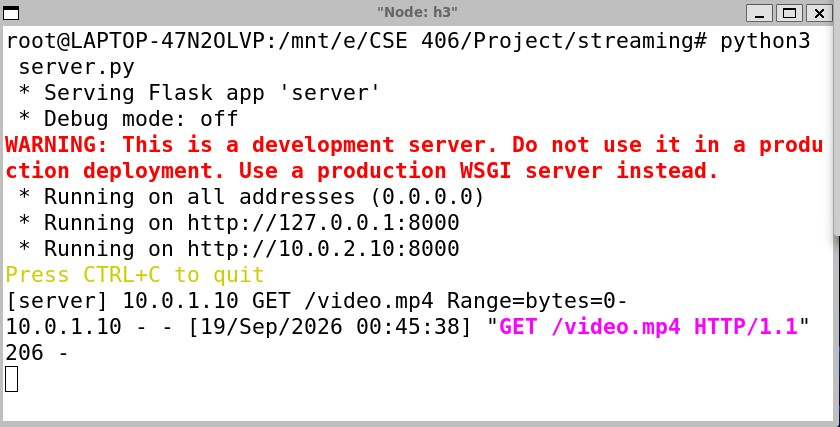
\includegraphics[width=\linewidth]{Images/h3_terminal_got_206_getrequest.jpg}
  \caption{Server (h3): incoming request, 206 response}
\end{subfigure}
\hfill
\begin{subfigure}{0.48\textwidth}
  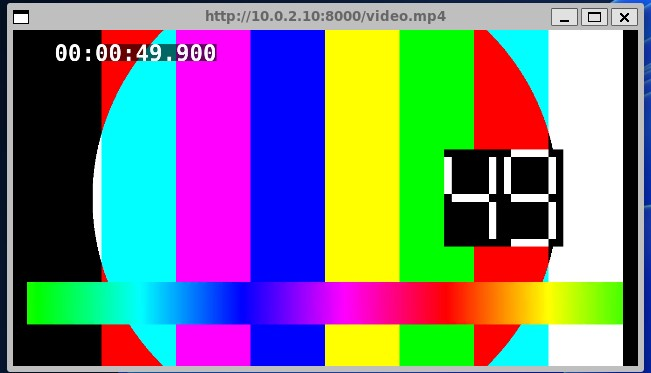
\includegraphics[width=\linewidth]{Images/video_player_window.jpg}
  \caption{Client: normal playback, before the attack}
\end{subfigure}
\caption{Baseline, before the attack: the server logging the client's
request (left) and the client playing normally (right).}
\label{fig:before}
\end{figure}

\begin{figure}[h]
\centering
\begin{subfigure}{0.48\textwidth}
  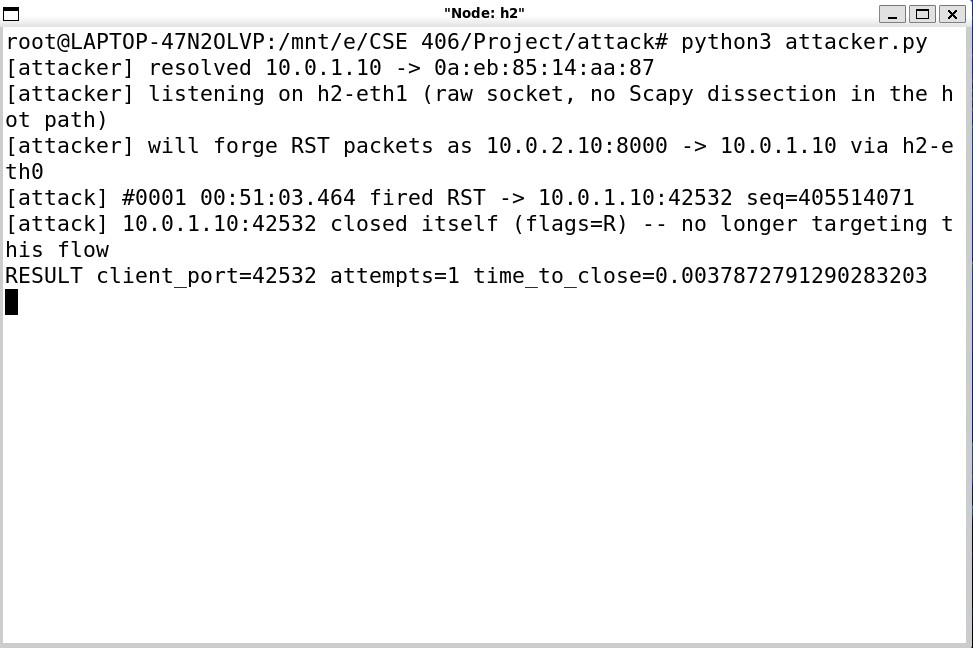
\includegraphics[width=\linewidth]{Images/attacker_firing_rst_pkt.jpg}
  \caption{Attacker (h2): fires one forged RST, connection closes immediately}
\end{subfigure}
\hfill
\begin{subfigure}{0.48\textwidth}
  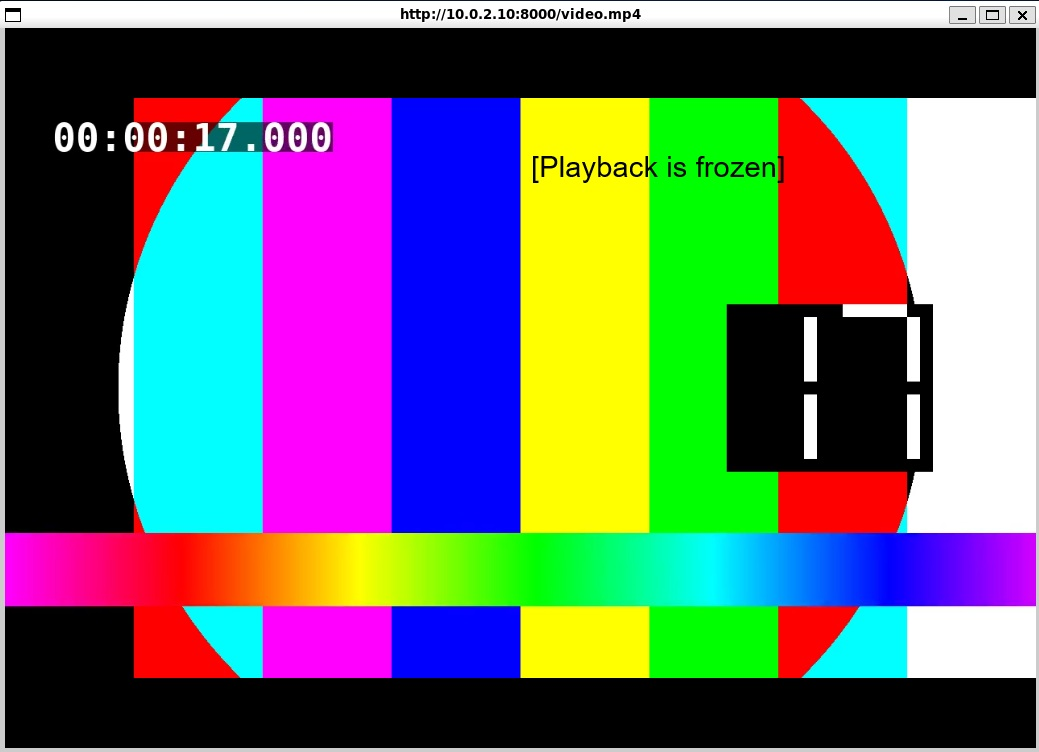
\includegraphics[width=\linewidth]{Images/video_player_window_frozen.jpg}
  \caption{Client: playback frozen at the moment of the attack}
\end{subfigure}
\caption{The attack: a single forged RST (left, note
\texttt{attempts=1}) kills the connection, and the client's playback
freezes at the same moment (right).}
\label{fig:during}
\end{figure}

\begin{figure}[h]
\centering
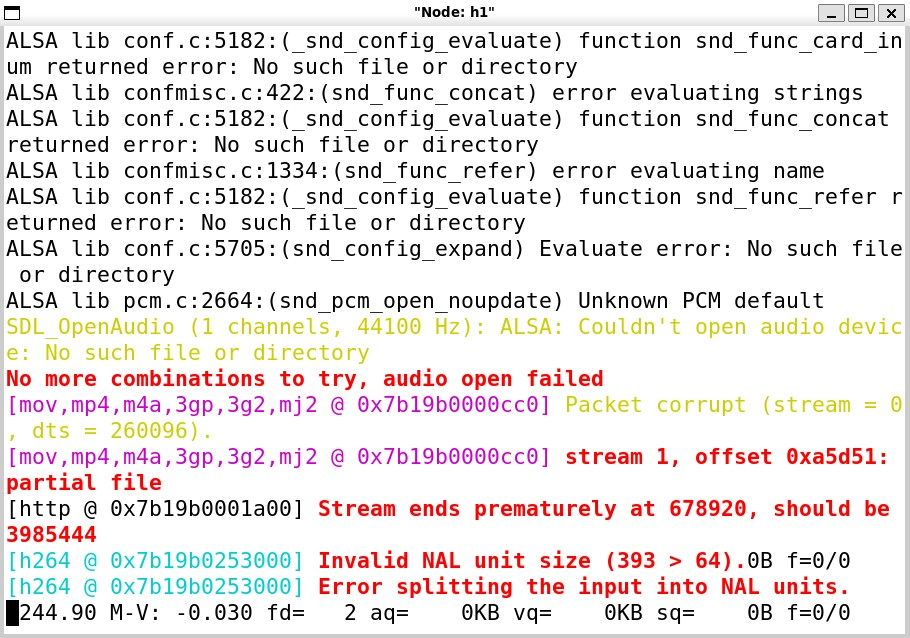
\includegraphics[width=0.85\textwidth]{Images/successful_attack_h1_terminal.jpg}
\caption{Victim's own terminal output (\texttt{ffplay}), confirming the
underlying transfer was severed abnormally partway through the file.}
\label{fig:victim-error}
\end{figure}

\paragraph{Attacker-side output.} A representative successful run
(Figure~\ref{fig:during}, left):
\begin{lstlisting}
[attacker] resolved 10.0.1.10 -> 0a:eb:85:14:aa:87
[attacker] listening on h2-eth1 (raw socket, no Scapy dissection in the hot path)
[attacker] will forge RST packets as 10.0.2.10:8000 -> 10.0.1.10 via h2-eth0
[attack] #0001 00:51:03.464 fired RST -> 10.0.1.10:42532 seq=405514071
[attack] 10.0.1.10:42532 closed itself (flags=R) -- no longer targeting this flow
RESULT client_port=42532 attempts=1 time_to_close=0.0037872791290283203
\end{lstlisting}
A single forged RST killed the connection. The client's own kernel then
generated a RST of its own back toward the server, for the next
already-in-flight real segment (arriving for a connection that no longer
exists locally) -- an independent, attacker-observable confirmation that
the kill worked, without needing to look at the victim's screen at all.

\paragraph{Victim-side output.} The player's own error output on a
successful attack (Figure~\ref{fig:victim-error}):
\begin{lstlisting}
[mov,mp4,m4a,3gp,3g2,mj2] Packet corrupt (stream = 0, dts = 260096).
[mov,mp4,m4a,3gp,3g2,mj2] stream 1, offset 0xa5d51: partial file
[http] Stream ends prematurely at 678920, should be 3985444
[h264] Invalid NAL unit size (393 > 64).
[h264] Error splitting the input into NAL units.
\end{lstlisting}
Only 678{,}920 of the expected 3{,}985{,}444 bytes ($\approx$17\%)
were received. This is the player's own confirmation that the underlying
TCP transfer was severed abnormally, not merely slow -- a slow-but-intact
download would not produce a ``partial file'' / ``ends prematurely''
error at all. (When \texttt{curl} is used instead of a GUI player for
scripted trials, the equivalent signal is a non-zero exit code, e.g.\
\texttt{56}, ``Recv failure: Connection reset by peer''.)

\paragraph{Server-side output.} The server's own log shows nothing
unusual:
\begin{lstlisting}
[server] 10.0.1.10 GET /video.mp4 Range=bytes=0-
10.0.1.10 - - [.../Sep/2026 ...] "GET /video.mp4 HTTP/1.1" 206 -
\end{lstlisting}
The server keeps sending data into a connection that is already dead
from the client's perspective, until its own transport-layer
error/timeout handling eventually notices. This asymmetry -- the
attacker targets the client, and the server has no direct indication
anything is wrong -- is a direct consequence of Attack A's design
(Section~\ref{sec:forge}).

\subsection{Quantitative Results}
\label{sec:quant}

To avoid relying on a single anecdotal demo run, we built an automated
experiment harness that drives the whole topology (server, attacker,
client) through $N$ repeated trials per condition, with success measured
objectively -- by comparing downloaded byte count against the video's
known full size, and by the client's own exit code -- rather than by
eyeballing a player. Each trial gives the download a head start
proportional to the estimated total transfer time before starting the
attacker, modeling an attacker that gains on-path visibility partway
through an already-flowing stream (as the ARP-spoofing precondition
would produce in practice), rather than one present since before the TCP
handshake.

Table~\ref{tab:sweep} reports the attack's success rate and mean
attempts-to-kill across a range of WAN bandwidths (20 trials per
condition, defense disabled).

\begin{table}[h]
\centering\small
\begin{tabular}{lccc}
\toprule
WAN bandwidth & Est.\ segment gap & Success rate & Mean attempts \\
\midrule
1 Mbit/s   & $\approx$24\,ms   & 100\%          & 1 \\
5 Mbit/s   & $\approx$4.8\,ms  & 100\% (20/20)  & 1.0 \\
12 Mbit/s  & $\approx$1.9\,ms  & 100\% (20/20)  & 1.05 \\
20 Mbit/s  & $\approx$1.2\,ms  & 100\% (20/20)  & 1.05 \\
50 Mbit/s  & $\approx$0.46\,ms & 100\% (20/20)  & 1.0 \\
100 Mbit/s & $\approx$0.23\,ms & \textbf{0\% (0/11)} & --- \\
\bottomrule
\end{tabular}
\caption{Attack success rate vs.\ WAN bandwidth, defense disabled.}
\label{tab:sweep}
\end{table}

We also captured packets directly on the victim to verify \emph{why}
the attack wins when it does: converting the forged RST's raw sequence
number back to the connection's relative byte offset shows it lands
exactly on the real stream's current boundary every time (never a
guess), and its arrival consistently precedes the real next segment by
a small but measurable margin (observed margins: 5.5\,ms, 10\,ms, and
3.2\,ms across three captured examples) -- a direct, measured
demonstration of the attacker's short-LAN-path-vs-long-WAN-path
advantage described in Section~\ref{sec:impl}.

\subsection{Expected vs.\ Observed Outcome, and Where They Differ}
\label{sec:diverge}

For the great majority of tested conditions (WAN bandwidths from 1 to
50\,Mbit/s, which covers everything from a poor mobile connection to a
high-quality stream), the observed outcome matched the expected outcome
exactly: the attack succeeded, essentially deterministically, in a
single shot per trial.

Two points are worth reporting explicitly because the observed outcome
did \emph{not} simply match expectations on the first attempt, and
understanding why is itself informative.

\paragraph{Divergence 1: implementation latency, not network conditions,
was the first real bottleneck.}
\label{sec:latency}
An initial version of the attacker used a well-known Python packet
library (Scapy) for both sniffing and crafting packets. Under automated,
repeated trials, this version showed a puzzling bimodal pattern: some
connections died in exactly one shot, while others fired 600+ times
across an entire streaming session and \emph{never} landed a single hit
-- not the smoothly probabilistic behavior the design predicted.
Packet-level diagnosis (a synchronized capture on the victim, comparing
the timestamp of each forged RST against the real segment it was racing)
found the actual cause: Scapy's per-packet object-construction overhead
was, on average, close to or above the real inter-segment gap on the
shaped WAN link ($\approx$24\,ms at 1\,Mbit/s). Once a single shot
happened to be slow, a processing backlog began accumulating and never
shrank back down -- a textbook unstable queue -- so the attacker ended
up reacting to progressively staler packets for the rest of the
connection's life, with reaction latency measured climbing from
27\,ms to over 16 \emph{seconds} across one losing trial.

This was fixed by rewriting the attacker to use raw \texttt{AF\_PACKET}
sockets with hand-rolled header parsing/construction (avoiding Scapy's
per-packet overhead), and by always processing the newest queued packet
rather than the oldest (bounding the worst case to one stale cycle
instead of an ever-growing backlog). After this fix, measured reaction
latency dropped to 0.1--10\,ms (typically sub-millisecond), and the
attack's behavior across repeated trials became the near-deterministic
one-shot success reported in Table~\ref{tab:sweep}. In short: the
initial divergence between expected and observed behavior was not a
flaw in the attack's design, but an artifact of Python/Scapy's
processing overhead exceeding the available race margin -- once that
overhead was removed, observed behavior matched the design's prediction.

\paragraph{Divergence 2: the race flips at unrealistically high
bandwidth.} At 100\,Mbit/s, the observed success rate dropped to 0\%
(0/11 trials) -- the opposite of the near-100\% outcome at every lower
bandwidth. This is explained directly by the same race-margin model: at
100\,Mbit/s the real segment gap shrinks to roughly 0.23\,ms, which is
now comparable to or below the attacker's own (already-optimized)
processing latency. The attacker's structural, topological advantage
(one LAN hop vs.\ a router-mediated WAN path) is necessary but not
sufficient once the legitimate traffic itself is moving faster than the
attacker's software can plausibly react. This is not a contradiction of
the attack's design -- the design was explicit from the start that
success depends on winning a race, not on a guaranteed exploit -- but it
is a concrete, measured boundary of where that race is actually won or
lost, and 100\,Mbit/s is well outside the range of realistic video
streaming bitrates, so it does not undermine the attack's practical
effectiveness.

% =======================================================================
\section{Defense Mechanism}
\label{sec:defense}
% =======================================================================

\subsection{Design}

\paragraph{Rejected approach: router-side ingress filtering.} An initial
idea was to drop, at the router, any packet claiming to be from the
server but arriving on the router's LAN-facing interface -- a genuine
server packet could only arrive via the WAN side. This fails
\emph{topologically}, not merely as weak policy: the forged RST travels
attacker $\to$ switch $\to$ client entirely within the LAN, since its
destination (the client) is on the local subnet. It never reaches the
router's LAN interface at all, so a router-side rule is not on this
attack's path and cannot see the malicious packet.

\paragraph{Chosen approach: switch-side IP Source Guard.} Every
attacker-to-victim frame must physically pass through the shared LAN
switch, which makes it the correct choke point. Real switches implement
IP Source Guard by binding each port to the IP/MAC pair learned via DHCP
snooping, then dropping any frame on that port whose source IP does not
match the binding. Since the attacker's real IP is known by construction
in our emulated topology, we install the equivalent access-control rule
directly on the Open vSwitch switch:
\begin{lstlisting}
ovs-ofctl add-flow s1 "priority=100,in_port=<attacker's port>,
  ip,nw_src=10.0.2.10,actions=drop"
\end{lstlisting}
This rule drops only IPv4 packets that forge the server's address while
entering on the attacker's specific switch port; the attacker's own real
traffic (using its own IP) and all ARP traffic are unaffected, and the
rule does not interfere with the mirror-based visibility mechanism from
Section~\ref{sec:visibility} -- the defense stops forged \emph{delivery}
of the attack packet, not the (separately assumed) ARP-spoofing
visibility precondition itself.

\subsection{Defense Evaluation: Does It Work as Expected?}

The expectation was that this defense should reduce the attack's success
rate to 0\%, regardless of network bandwidth, since it operates as a
deterministic access-control check at the switch rather than depending
on any timing race. Table~\ref{tab:defense} reports the measured
before/after comparison across the same repeated-trial methodology used
in Section~\ref{sec:quant}.

\begin{table}[h]
\centering\small
\begin{tabular}{lcc}
\toprule
WAN bandwidth & Defense off (success rate) & Defense on (success rate) \\
\midrule
5 Mbit/s   & 100\% & \textbf{0\%} \\
12 Mbit/s  & 100\% & \textbf{0\%} \\
20 Mbit/s  & 100\% & \textbf{0\%} \\
50 Mbit/s  & 100\% & \textbf{0\%} \\
\bottomrule
\end{tabular}
\caption{Attack success rate with the defense disabled vs.\ enabled, 20 trials per condition.}
\label{tab:defense}
\end{table}

The observed outcome matched the expectation exactly: with the defense
enabled, every trial across every tested bandwidth resulted in a full,
uninterrupted download -- the attacker fired hundreds of forged RSTs per
trial (since it has no awareness of the defense and simply keeps trying)
and none of them reached the victim.

\begin{figure}[h]
\centering
\begin{subfigure}{0.48\textwidth}
  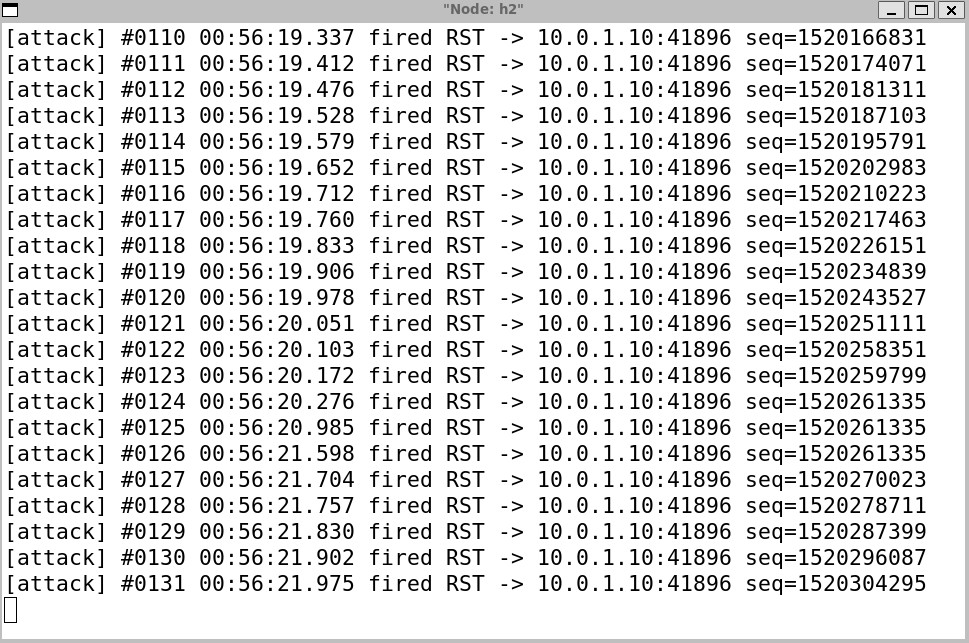
\includegraphics[width=\linewidth]{Images/defense_on_failedattack_h2_terminal.jpg}
  \caption{Attacker's terminal: 130+ forged RSTs fired, none succeed}
\end{subfigure}
\hfill
\begin{subfigure}{0.48\textwidth}
  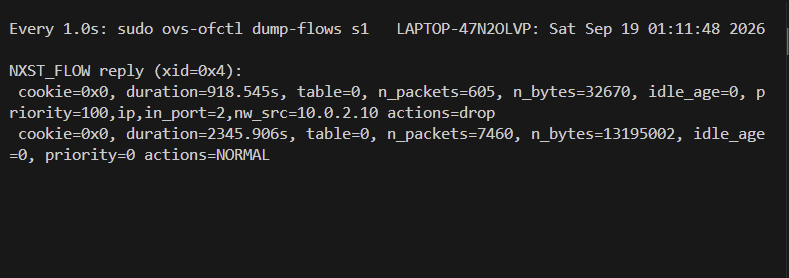
\includegraphics[width=\linewidth]{Images/dump_flows_drop_counter.png}
  \caption{Switch's own flow table: the drop rule's \texttt{n\_packets} counter}
\end{subfigure}
\caption{Defense evidence: the attacker's own terminal (left) and the
switch's flow-rule counters (right, \texttt{ovs-ofctl dump-flows s1},
refreshed live via \texttt{watch}).}
\label{fig:defense-evidence}
\end{figure}

Figure~\ref{fig:defense-evidence} (left) shows the attacker's terminal
well past its 100th attempt against a single connection, still firing
and still failing -- exactly the behavior expected of a switch-level
drop rather than a timing loss (a timing loss would still occasionally
succeed; a hard drop never does). We confirmed the mechanism directly,
not just its effect, by inspecting the switch's own flow-rule counters
(Figure~\ref{fig:defense-evidence}, right): the installed rule
(\texttt{priority=100,ip,in\_port=2,nw\_src=10.0.2.10 actions=drop})
shows \texttt{n\_packets=605} and climbing under \texttt{watch}, in
step with the attacker's own attempt count -- direct confirmation that
the forged packets are being matched and dropped at the switch, not
failing to arrive for some unrelated reason. Unlike the attack itself
(Section~\ref{sec:diverge}), the defense's effectiveness does not depend
on network speed at all, since it is a deterministic access-control
check rather than a timing race --
this is exactly the behavior expected of the design.

% =======================================================================
\section{Discussion, Scope, and Limitations}
\label{sec:discussion}
% =======================================================================

The threat model and assumptions stated in Section~\ref{sec:threat} bound
the scope of what was implemented and evaluated. In particular: ARP
spoofing (the on-path visibility precondition) was assumed already
satisfied rather than implemented, since it is a separately assigned
project tool; only Attack A (forged RST to the client) was implemented
and evaluated, not the converse Attack B; and the attacker deliberately
never suppresses or delays legitimate traffic, only observes and
injects.

Within that scope, some further limitations are worth noting. The race
behavior in Section~\ref{sec:quant} was characterized only for the
specific topology and bandwidth/delay range tested; real-world WAN paths
have more variable delay and jitter than our shaped emulation, which
could shift the exact bandwidth at which the race flips (Divergence 2,
Section~\ref{sec:diverge}) in either direction. RFC 5961's challenge-ACK
behavior for an \emph{inexact} (guessed, rather than sniffed) sequence
number was discussed conceptually during design but not separately
implemented or measured, since our attacker always uses the exact
sniffed value and so never exercises that code path. Possible
extensions include implementing Attack B, an off-path sequence-guessing
variant (to concretely exercise the challenge-ACK path RFC 5961
provides), and TTL-based anomaly detection as an additional, complementary
defense layer.

% =======================================================================
\section{Conclusion}
\label{sec:conclusion}
% =======================================================================

We implemented, from scratch, a working TCP reset attack that reliably
interrupts video streaming under realistic network conditions, using
only self-crafted raw-socket code for both sniffing and packet
construction. We measured its actual success rate and behavior across a
range of network conditions rather than relying on a single demo run,
and explicitly identified and explained the two cases where the observed
outcome diverged from the naive expectation: an initial
implementation-latency bottleneck (fixed, and confirmed fixed by
re-measurement) and a genuine, expected-in-principle race-margin
boundary at unrealistically high bandwidth. We further designed,
implemented, and evaluated a switch-side IP Source Guard countermeasure
that reduces the attack's success rate from 100\% to 0\%, and confirmed
that this defense behaves exactly as expected -- deterministically,
independent of network speed -- across every tested condition.

\bigskip
\noindent\textbf{Contribution split.}
\begin{center}
\begin{tabular}{@{}p{3.2cm}p{9.5cm}@{}}
\toprule
Member & Contribution \\
\midrule
2105094: Omar Abdur Razzaque & \fillin{describe this member's actual contribution} \\[0.3em]
2105104: Rubaiyat-E-Zaman & \fillin{describe this member's actual contribution} \\
\bottomrule
\end{tabular}
\end{center}

% =======================================================================
\section*{References}
% =======================================================================
\begin{enumerate}[leftmargin=1.5em]
\item RFC 793 --- Transmission Control Protocol.
\item RFC 5961 --- Improving TCP's Robustness to Blind In-Window Attacks.
\item Ishtiaq, Faruk, Hossain --- \emph{TCP Reset Attack on Video Streaming}, NSysS 2019 poster (BUET).
\item Watson, P. --- \emph{Slipping in the Window: TCP Reset Attacks}.
\item \fillin{any additional references you used}
\end{enumerate}

\end{document}
